\documentclass[a4paper,12pt]{article}
\usepackage{mypackages}
\usepackage{macros}

\begin{document}

\title{Cheat Sheet - LaTex}
\author{N. Bancel}
\date{Septembre 2024}
\maketitle

\section{Figures}

\begin{figure}[H]
  \centering
  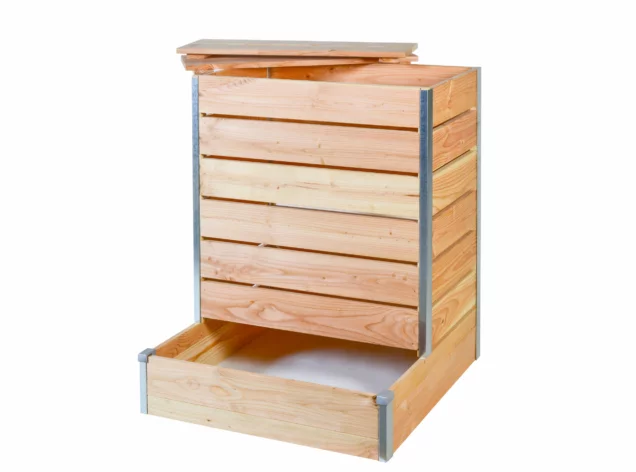
\includegraphics[width=0.3\linewidth]{lombri.jpg}
  \caption{\label{} Blablabla}
\end{figure}

Hyperlinks : 

\href{http://www.overleaf.com}{Something Linky} 

\section{Enumération / Listes}

\begin{enumerate}[noitemsep]
  \item Item 1
  \item Item 2
  \item Item 3
\end{enumerate}

\section{Boxes}

\begin{tcolorbox}[colback=red!10!white, colframe=red!75!black, title=PAR COEUR]
  Voici la définition de blablabla
\end{tcolorbox}


\begin{tcolorbox}[colback=green!10!white, colframe=green!75!black, title=Définition : xxx]
  Voici la définition de blablabla
\end{tcolorbox}

\begin{tcolorbox}[colback=blue!10!white, colframe=blue!75!black, title=Exemples - Application]
  Voici un exemple de blablabla
\end{tcolorbox}

\section{Tableaux}

\begin{tabular}{SS}
  \toprule
  {Heading 1} & {Heading 2} \\
  \midrule
  {Composant 1} & {Valeur 1} \\
  {Composant 2} & {Valeur 2} \\
  \bottomrule
\end{tabular}

\end{document}
